% -----------------------------------------------------------------
% Document class: Article
\documentclass[ a4paper, twoside, 11pt]{article}
\usepackage{../../../macros-general}
\usepackage{../../../macros-article}
% Number of the handout, quiz, exam, etc.
\newcommand{\numero}{05}
\setcounter{numero}{\numero}

% -----------------------------------------------------------------
\begin{document}
\allowdisplaybreaks

\begin{center}
\Large Mec\'anica Vectorial (MECG-1001): Trabajo Aut\'onomo \numero \\[2ex]
\small \textbf{Semestre:} 2017-2018 T\'ermino II \qquad
\textbf{Instructor:} Luis I. Reyes Castro \qquad
\textbf{Paralelo:} 08
\end{center}
\fullskip

% =============================================
\begin{problem}
\textbf{[4 Puntos]} La barra uniforme $BD$ de 250 mm y 5 kg de masa est\'a conectada como se muestra al disco $A$ y a un collar\'in de masa despreciable, el cual puede deslizarse libremente a lo largo de una barra vertical. Si se sabe que el disco $A$ gira en sentido contrario al de las manecillas del reloj a la velocidad constante de 500 rpm, determine, para el caso cuando $\theta = 90\deg$, \textit{(i)} la aceleraci\'on angular de la barra y \textit{(ii)} la reacci\'on en $D$. 

\begin{figure}[htb]
\centering
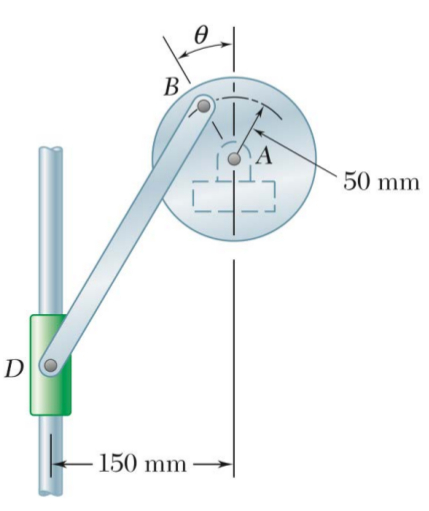
\includegraphics[width=0.4\textwidth]{problema-1.jpg} \quad
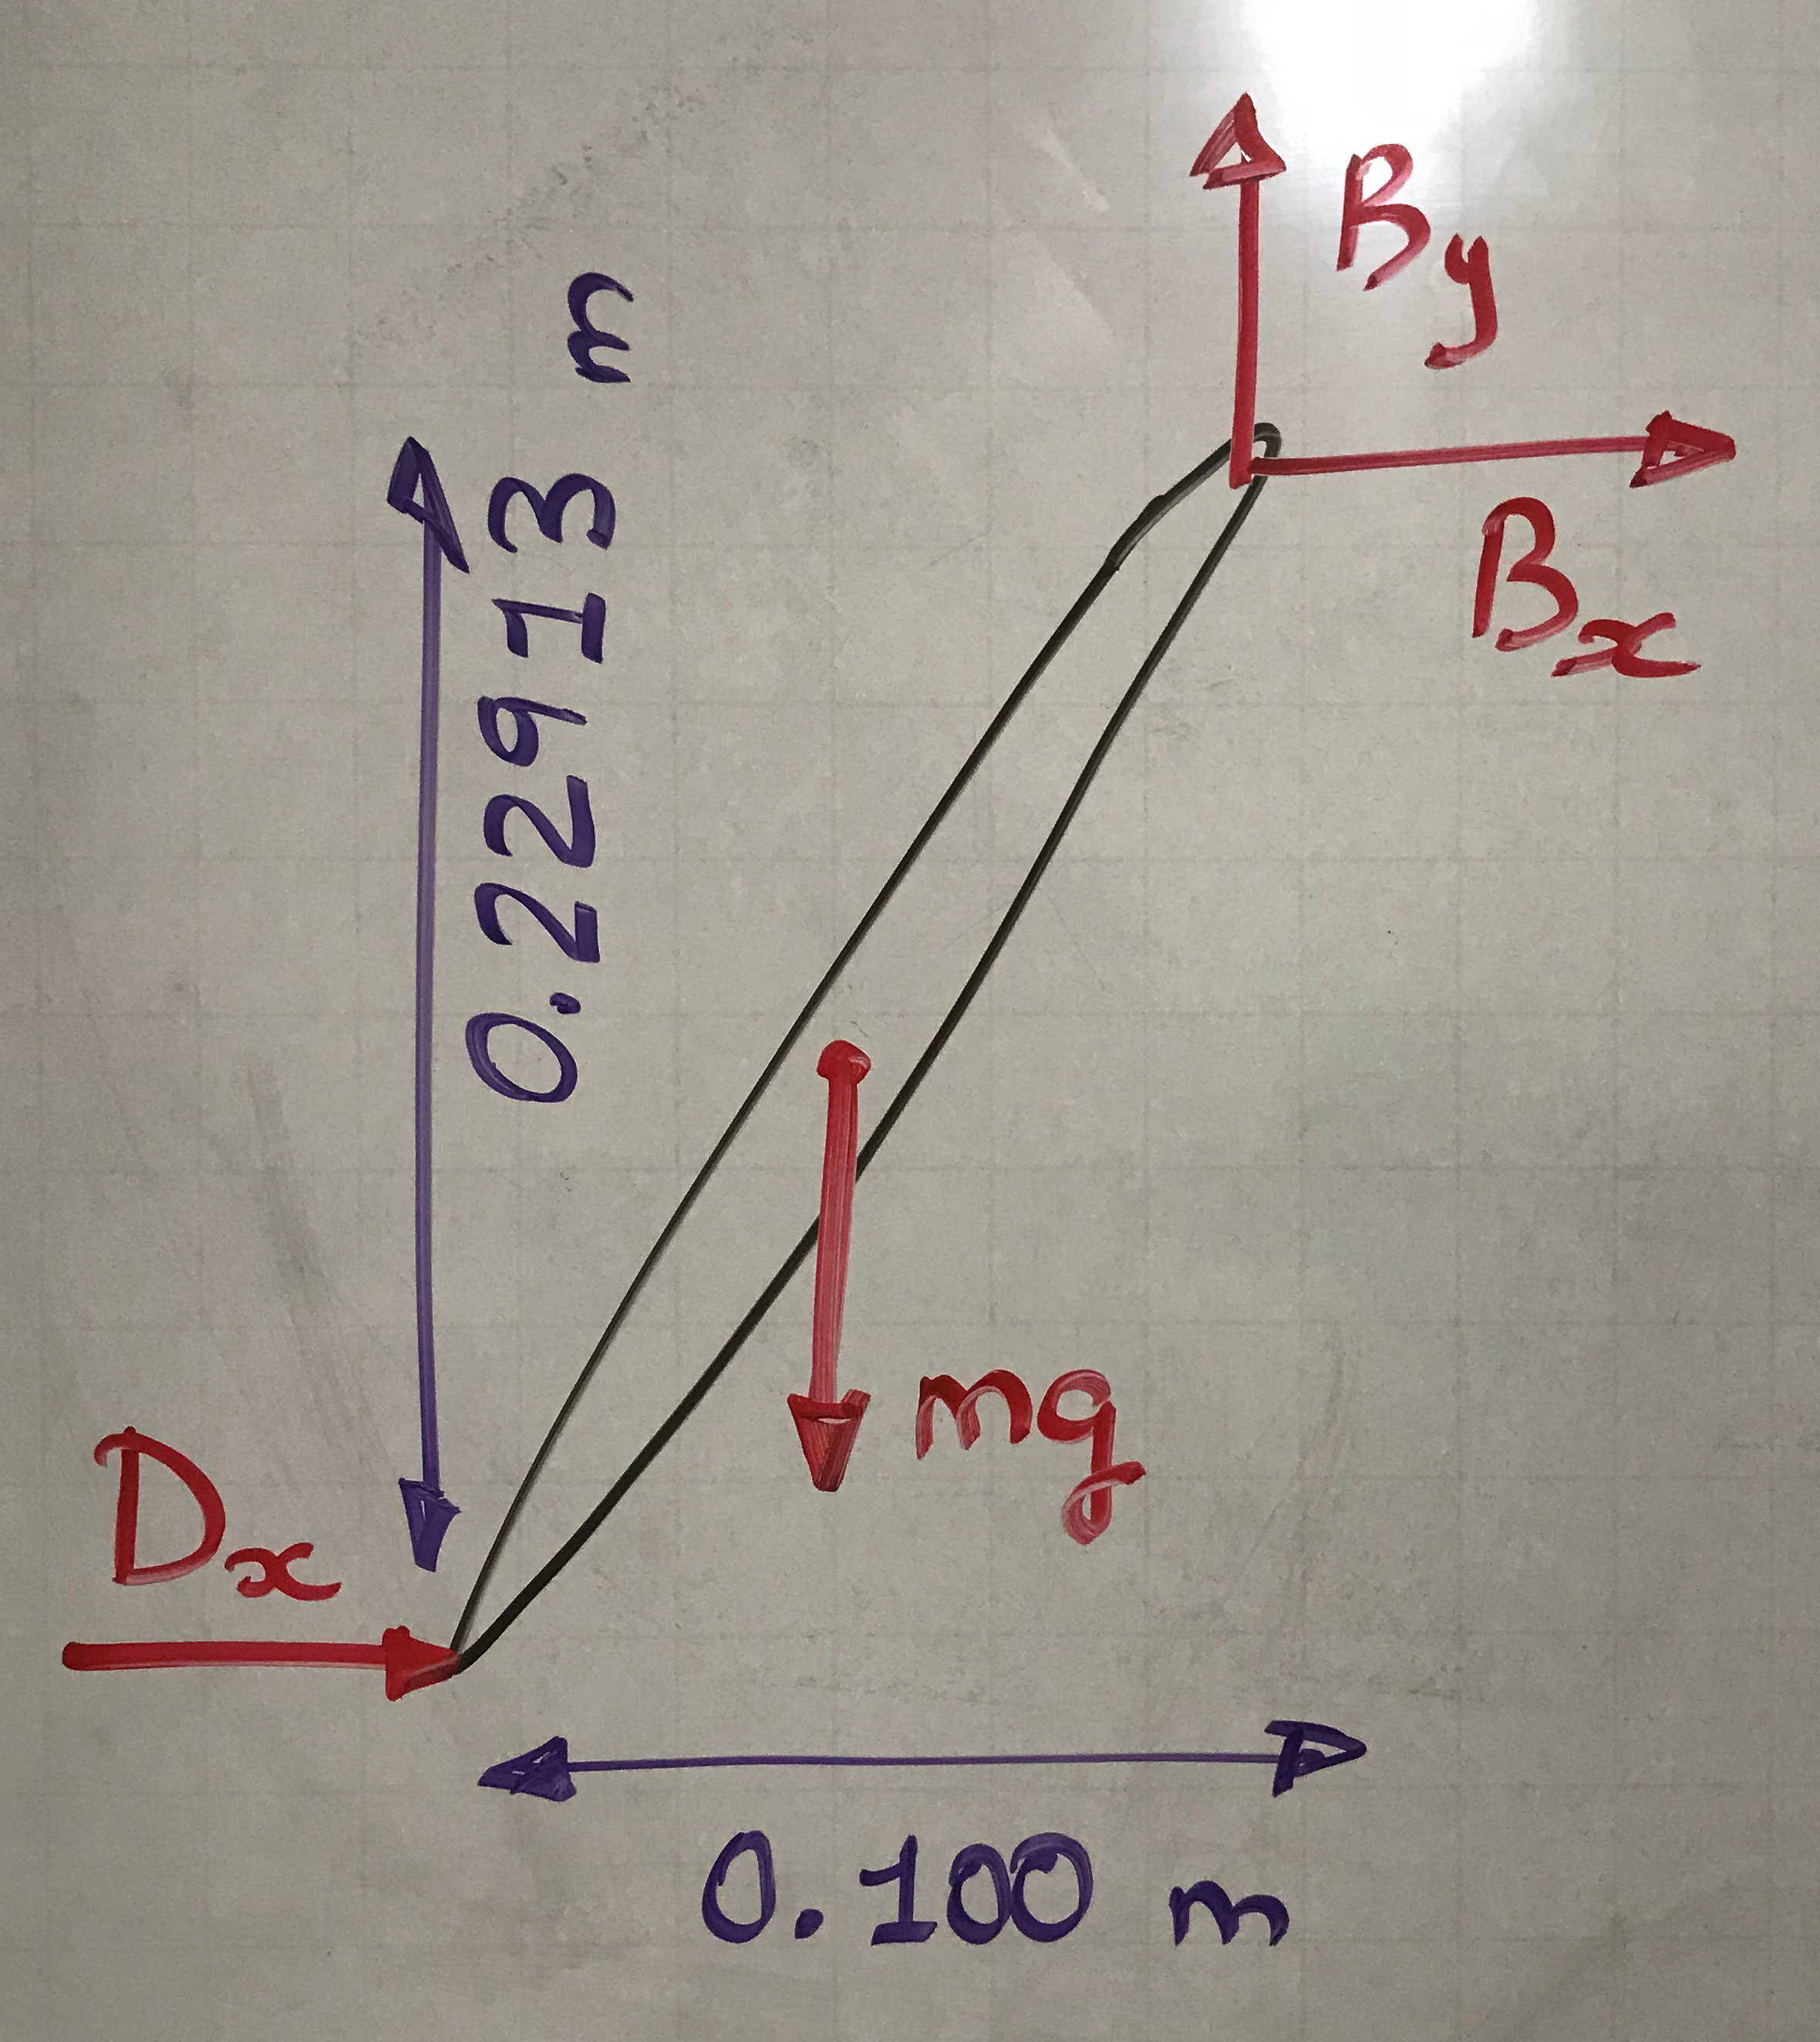
\includegraphics[width=0.4\textwidth]{problema-1_DCL.jpg}
\end{figure}

\emph{Soluci\'on:} Empezamos tomando datos: 
\begin{align*}
m \; & = \; 5 \; \text{kg} \qquad \Longrightarrow \qquad
m \, g \; = \; 49.05 \; \text{N} \\
I_G \; & = \; (1/12) \, m \, \ell^2 \; = \; 0.026 \; \text{kg-m\tsup{2}} \\
\vec{r_{BD}} \; & = \; ( \, -0.100, \, -0.2291 \, ) \\
\vec{r_{GB}} \; & = \; ( \, +0.050, \, +0.1145 \, ) \\
\vec{r_{GD}} \; & = \; ( \, -0.050, \, -0.1145 \, ) \\
\vec{r_{AB}} \; & = \; ( \, -0.050, \, 0 \, ) \\
\vec{\omega_{AB}} \; & = \; +52.36 \; \uvec{k} \; \text{rad/s}
\end{align*}
Primero calculamos $\vec{v_B}$ y $\vec{a_B}$. 
\begin{align*}
\vec{v_B} \;
& = \; \vec{v_A} + \vec{\omega_{AB}} \cross \vec{r_{AB}}
\; = \; \vec{0} + \vec{\omega_{AB}} \cross \vec{r_{AB}} \\
& = \; ( \, 0, \, -2.618 \, ) \; \text{m/s} \\
\vec{a_B} \;
& = \; \vec{a_A} + \vec{\alpha_{AB}} \cross \vec{r_{AB}} + \vec{\omega_{AB}} \cross ( \vec{\omega_{AB}} \cross \vec{r_{AB}} ) \\
& = \; \vec{0} + \vec{0} \cross \vec{r_{AB}} - \omega_{AB}^2 \, \vec{r_{AB}} \\
& = \; ( \, +137.08, \, 0 \, ) \; \text{m/s\tsup{2}}
\end{align*}
Luego, reconociendo que $\vec{v_D} = +v_D \, \uvec{j}$, tenemos: 
\begin{align*}
\vec{v_D} \;
& = \; \vec{v_B} + \vec{\omega_{BD}} \cross \vec{r_{BD}} \\
\Longrightarrow \; \colvec{0}{+v_D} \;
& = \; \colvec{0}{-2.618} +
\colvec{ +0.2291 \, \omega_{BD}}{ -0.100 \, \omega_{BD}} \\
\Longrightarrow \; 0 & = \; +0.2291 \, \omega_{BD} \qquad
\Longrightarrow \; \vec{\omega_{BD}} \; = \; \vec{0} \; \text{rad/s}
\end{align*}
Similarmente, reconociendo que $\vec{a_D} = +a_D \, \uvec{j}$, tenemos: 
\begin{align*}
\vec{a_D} \;
& = \; \vec{a_B} + \vec{\alpha_{BD}} \cross \vec{r_{BD}} + \vec{\omega_{BD}} \cross ( \vec{\omega_{BD}} \cross \vec{r_{BD}} ) \\
& = \; \vec{a_B} + \vec{\alpha_{BD}} \cross \vec{r_{BD}} + \vec{0} \\
\Longrightarrow \; \colvec{0}{+a_D} \;
& = \; \colvec{+137.08}{0} +
\colvec{ +0.2291 \, \alpha_{BD}}{ -0.100 \, \alpha_{BD}} \\
\Longrightarrow \; 0 & = \; +137.08 + 0.2291 \, \omega_{BD} \qquad
\Longrightarrow \; \vec{\alpha_{BD}} \; = \; -598.34 \; \uvec{k} \; \text{rad/s\tsup{2}}
\end{align*}
Consecuentemente: 
\begin{align*}
\vec{a_G} \;
& = \; \vec{a_B} + \vec{\alpha_{BD}} \cross \vec{r_{BG}} + \vec{\omega_{BD}} \cross ( \vec{\omega_{BD}} \cross \vec{r_{BG}} ) \\
& = \; \vec{a_B} + \vec{\alpha_{BD}} \cross \vec{r_{BG}} + \vec{0} \\
\Longrightarrow \; 
\colvec{ (\vec{a_G})_x}{ (\vec{a_G})_y} & =
\; \colvec{+137.08}{0} +
\colvec{ +0.2291 \, (-598.34)}{ -0.100 \, (-598.34)} \; \approx \; \colvec{0.0}{+59.8} \; \text{m/s\tsup{2}}
\end{align*}
Ahora bosquejamos el diagrama de cuerpo libre (DCL) de la barra $AB$, tal como se muestra en la fotograf\'ia a la derecha de la figura del problema. Las sumatorias de fuerzas y momentos externos son: 
\begin{align*}
m \, (\vec{a_G})_x \; & = \; B_x + D_x \\
& \Longrightarrow \quad 0 \; = \; B_x + D_x
\quad \Longrightarrow \quad B_x \; = -D_x \\
m \, (\vec{a_G})_y \; & = \; B_y - mg \\
& \Longrightarrow \quad
B_y \; = \; m \, ( \, (\vec{a_G})_y + g \, )
\; = \; 348.05 \; \text{N} \\
I \, \alpha \; & = \; +0.1145 \, ( +D_x - B_x ) + 0.050 \, B_y \\
& \Longrightarrow \quad
(0.026)(-598.34) \; = \; +0.1145(+2 D_x) + 0.050 (348.05) \\
& \Longrightarrow \quad
D_x \; = \; -143.93 \; \text{N}
\end{align*}
En conclusi\'on: 
\[
\vec{\alpha_{BD}} \; = \; -598.34 \; \uvec{k} \; \text{rad/s\tsup{2}}
\qquad \qquad \qquad
\vec{D} \; = \; ( \, -143.93, \, 0 \, ) \; \text{N}
\]
\QED

\end{problem}
\fullskip

% =============================================
\begin{problem}
\textbf{[4 Puntos]} La caja uniforme $C$ de 100 kg descansa sobre el piso del elevador donde el coeficiente de fricci\'on est\'atica es $\mu = 0.4$. Determine la mayor aceleraci\'on angular inicial $\alpha$, comenzando desde el reposo en $\theta = 90\deg$, sin causar deslizamiento de la caja. Suponga que no es posible que la caja se vuelque. 

\begin{figure}[htb]
\centering
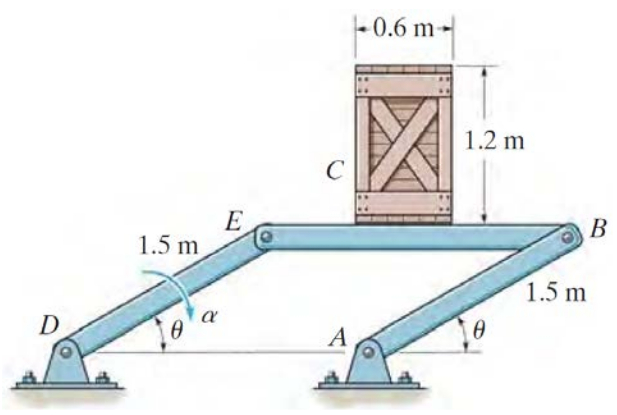
\includegraphics[width=0.6\textwidth]{problema-2.jpg}
\end{figure}

\emph{Soluci\'on:} Es evidente de la figura que la barra $EB$ sobre la cual descansa la caja est\'a en translaci\'on curvil\'inea, \ie $\vec{\omega_{EB}} = \vec{0}$ rad/s y $\vec{\alpha_{EB}} = \vec{0}$ rad/s. Esto implica que: 
\[
\vec{a_C} \; = \; \vec{a_B} + \vec{\alpha_{EB}} \cross \vec{r_{BC}} + \vec{\omega_{EB}} \cross ( \vec{\omega_{EB}} \cross \vec{r_{BC}} ) \\
\vec{a_B} + \vec{0} + \vec{0} \; = \; \vec{a_B}
\]
Adicionalmente, podemos reconocer que $\vec{\omega_{AB}} = \vec{\omega_{DE}} = \vec{0}$ y que $\vec{\alpha_{AB}} = \vec{\alpha_{DE}} = -\alpha \, \uvec{k}$. Consecuentemente: 
\begin{align*}
\vec{a_C} \; = \; \vec{a_B} \;
& = \; \vec{a_A} + \vec{\alpha_{AB}} \cross \vec{r_{AB}} + \vec{\omega_{AB}} \cross ( \vec{\omega_{AB}} \cross \vec{r_{AB}} ) \\
& = \; \vec{0} + \vec{\alpha_{AB}} \cross \vec{r_{AB}} + \vec{0}
\; = \; +r_{AG} \, \alpha \, \uvec{i}
\end{align*}
Ahora, como nos han dicho que supongamos que la caja no se puede volcar, la podemos modelar como una part\'icula cuya aceleraci\'on es igual a $\vec{a_C}$. Entonces, suponiendo que la fuerza de fricci\'on $f = \mu \, N = \mu \, m \, g$ abastece para mover la caja, la sumatoria de fuerzas externas en el eje-$x$ para la misma es: 
\[
m \, (\vec{a_C})_x \; = \; \mu \, m \, g
\qquad  \Longrightarrow \qquad
r_{AG} \, \alpha \; = \; \mu \, g
\qquad  \Longrightarrow \qquad
\alpha \; = \; \frac{\mu \, g}{r_{AC}}
\]
De esta manera, la mayor aceleraci\'on angular inicial posible es:
\[
\alpha \; = \; \frac{(0.4)(9.81)}{1.5}
\; = \; 2.616 \; \text{rad/s\tsup{2}}
\]

\emph{Nota:} Es curioso el hecho de que la respuesta no depende en la masa de la caja. 

\QED

\end{problem}
\fullskip

\end{document}